\newpage
\thispagestyle{empty}
% Se modifica la geometría (los márgenes) de la página y se coloca en formato horizontal:
\newgeometry{top=10mm, bottom=10mm, left=12mm, right=12mm}
\begin{landscape}

\subsubsection{Adjusted Rand Index Entre los Diferentes Clusters Obtenidos}

En la siguiente figura se muestra el \textit{Adjusted Rand Index} entre los diferentes clusters obtenidos. 

\begin{figure}[H]
    \centering
    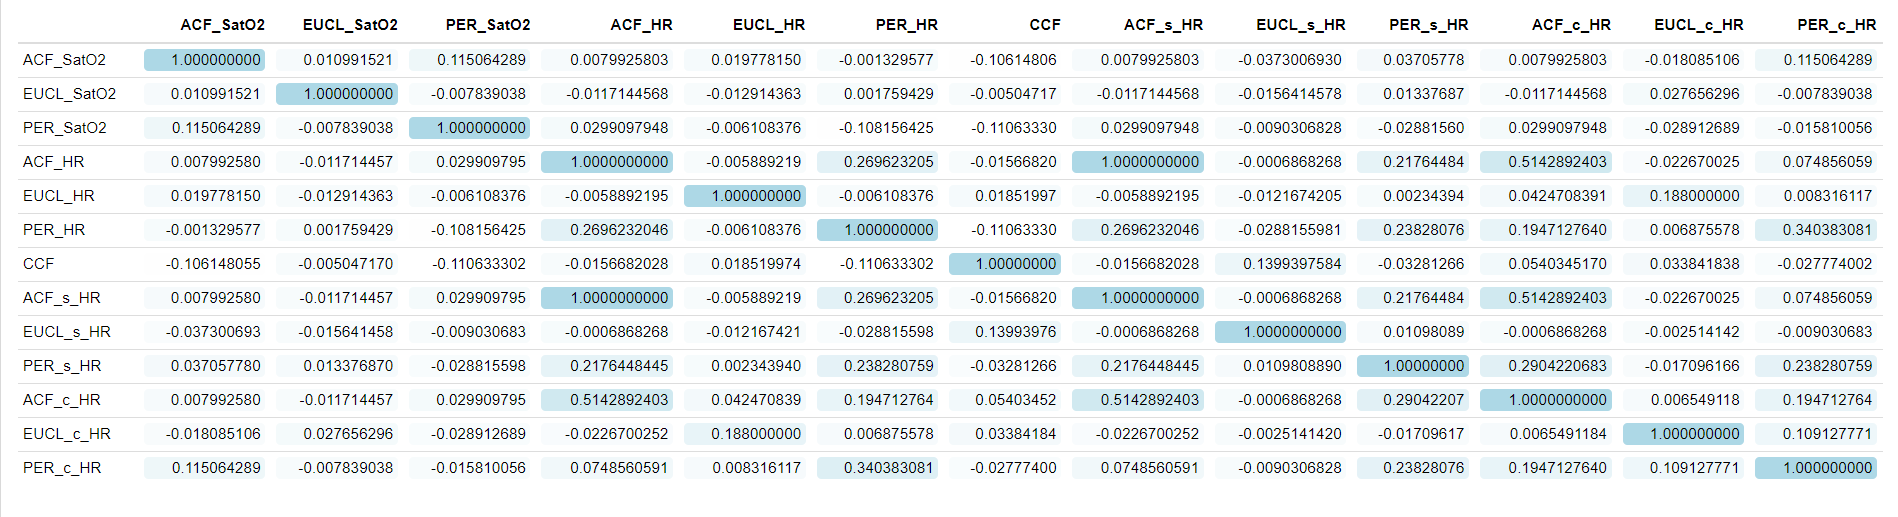
\includegraphics[scale=0.65]{img/adj-rand-index.png}
    \caption{Adjusted Rand Index entre los diferentes clusters obtenidos}
    \label{fig:Adj-Rand-Index}
\end{figure}

\textbf{Índice para entender la figura \ref{fig:Adj-Rand-Index}:}
\begin{description}
  \item[\texttt{HR:}] Frecuencia Cardíaca
  \item[\texttt{s\_HR:}] Frecuencia Cardíaca Escalada
  \item[\texttt{c\_HR:}] Frecuencia Cardíaca Transformada a Cuantiles
  \item[\texttt{SatO2:}] Saturación de Oxígeno
  \item[\texttt{s\_SatO2:}] Saturación de Oxígeno Escalada
  \item[\texttt{PER:}] Valores del peridiograma
  \item[\texttt{ACF:}] Valores de la Función de Autocorrelación (FAC)
  \item[\texttt{CCF:}] Valores de la Función de Correlación Cruzada (FCC) entre Frecuencia Cardíaca y Saturación de Oxígeno
\end{description}


\end{landscape}
\restoregeometry


